% Provenance (never printed): see sources/outline_sources.md (Year 2: ancient massifs,
% Caledonian and Variscan belts; the Wilson cycle; supercontinents). Caledonian phases after
% McKerrow, Mac Niocaill and Dewey (2000) and Schiffer et al. (2020); the Wilson cycle after
% Chenin et al. (2018) and Schiffer et al. (2020); the Variscan belt after Faure (2024);
% supercontinents after Nance (2022); Siccar Point after the IUGS Geoheritage description.
% Model ocean and supercontinent chart from figdata/bachelor-2/wilson.py. Exercise and problem
% values in the Book 4 scratch calculator calc/ch15.py.
\chapter{प्राचीन पुंजक और विल्सन चक्र}\label{ch:b2:wilson-cycle}

दक्षिण-पूर्वी स्कॉटलैंड के तट पर, सिकर पॉइंट पर, बलुआ पत्थर की धूसर परतें सीधी खड़ी हैं,
लाल बलुआ पत्थर के एक ढक्कन के नीचे जो समुद्र की ओर हल्का नत है। धूसर परतें आरंभिक सिल्यूरियन में
एक महासागर में जमी थीं, फिर उस महासागर के बंद होने पर वलित और विदलित हुईं; वे घिसकर
एक असमतल सतह बन गईं; उत्तर डेवोनियन में लाल बजरी ने उन्हें दबा दिया, और एक दूसरे,
अधिक मंद पर्वतजनन ने बारी आने पर लाल परतों को झुका दिया। एक खड़ी चट्टान एक ऐसे महासागर को अंकित करती है जो
लुप्त हो गया, एक ऐसी पर्वत-पट्टी को जो जा चुकी है, और अगली को भी। यह अध्याय ऐसे अभिलेखों को पढ़ता है,
उन्हें एक चक्र में एकत्र करता है जिसका महासागरीय द्रोणियाँ अनुसरण करती हैं, और पीछे हटकर सबसे लंबी लय को देखता है,
यानी \omterm{def:b2:wilson-cycle:supercontinent}{महामहाद्वीपों} का जुड़ना और टूटना।
% ledger: iugs:siccar-orogenies, iugs:siccar-point

\begin{recall}
\textbf{स्कूल की पुस्तकों से}: पैंजिया और उसका टूटना, \omterm{def:b2:wilson-cycle:supercontinent}{महामहाद्वीप}; असंगतियाँ;
अनाच्छादन दर, समस्थितिक प्रतिक्षेप, और अपनी नदियों द्वारा घिसी जाती पर्वतमाला का घातांकी
क्षय। \textbf{पुस्तक 3 (स्नातक वर्ष 1) से}: महाद्वीपीय दरारें, निष्क्रिय किनारे और
मध्य-महासागरीय कटक, पूर्ण और अर्ध प्रसार-दरें; क्षेपण और सक्रिय किनारे।
\textbf{\cref{ch:b2:crustal-melting} से \cref{ch:b2:himalaya-andes} तक}: \omterm{def:b2:crustal-melting:migmatite}{मिग्मेटाइट} और
ग्रेनाइट; \omterm{def:b2:alpine-orogen:orogen}{पर्वतजनक पट्टी}, \omterm{def:b2:alpine-orogen:ophiolite}{ओफ़ियोलाइट}, सीवन, \omterm{def:b2:alpine-orogen:nappes}{नैप}, \omterm{def:b2:alpine-orogen:foreland}{फ़्लिश} और \omterm{def:b2:alpine-orogen:foreland}{मोलास}, \omterm{def:b2:alpine-orogen:foreland}{अग्रभूमि द्रोणी}; \omterm{def:b2:himalaya-andes:types}{टक्कर-पट्टियाँ} और
एंडीज़-प्रकार की पट्टियाँ; \omterm{def:b2:himalaya-andes:thickening}{भूपर्पटीय स्थूलन}, एयरी मोटाई और \omterm{def:b2:himalaya-andes:collapse}{गुरुत्वीय निपात}।
\end{recall}

\begin{omfigure}
\centering
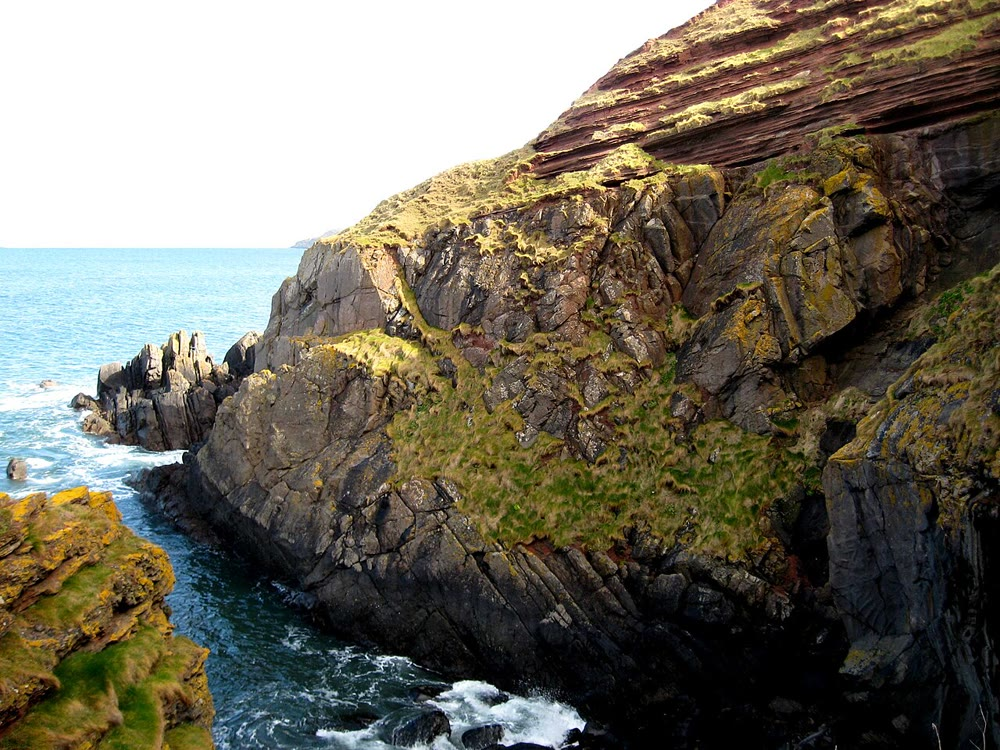
\includegraphics[width=0.64\linewidth]{images/book4/b2-15-siccar-point.jpg}
\par\smallskip{\small बिंदु के दक्षिण-पूर्व से सिकर पॉइंट: धूसर सिल्यूरियन
ग्रेवैक की लगभग ऊर्ध्वाधर परतें, जो कैलेडोनियाई पर्वतजनन में वलित हुईं, ऊपरी डेवोनियन की
मंद नत लाल परतों के नीचे। फ़ोटो: dave souza, 2008, CC BY-SA 4.0।}
\end{omfigure}
% ledger: iugs:siccar-orogenies

\section{अपनी जड़ों तक घिसी पट्टियाँ}\label{sec:b2:wilson-cycle:old}

पश्चिमी यूरोप और पूर्वी उत्तर अमेरिका को आल्प्स से कहीं अधिक पुरानी पर्वत-पट्टियाँ काटती हैं।
उनके शिखर जा चुके हैं, पर उनकी चट्टानें बची हैं। उनमें से तीन यहाँ मायने रखती हैं।

\emph{कैलेडोनियाई} पट्टी नॉर्वे से स्कॉटलैंड और आयरलैंड होते हुए न्यूफ़ाउंडलैंड और
उत्तरी ऐपलेशियन तक चलती है, और आगे पूर्वी ग्रीनलैंड और स्वालबार्ड तक। यह एक
महासागर, आयपेटस, का अभिलेख है, जो आरंभिक पैलियोज़ोइक में उत्तर-पश्चिम में लॉरेंशिया, यानी उत्तर
अमेरिका और ग्रीनलैंड के पूर्वज, और दक्षिण-पूर्व तथा पूर्व में बाल्टिका और एवलोनिया के बीच स्थित था।
उसके किनारों में लगभग 600 मिलियन वर्ष पहले दरार पड़ी थी; उसके बंद होने ने, कैम्ब्रियन से
डेवोनियन तक, टक्करों की एक पूरी शृंखला उत्पन्न की, जिससे कैलेडोनियाई पर्वतजनन कोई
200 मिलियन वर्षों में फैला है। यह शब्द एक स्थान और एक महासागर का नाम है, किसी आयु का नहीं।
% ledger: mckerrow00:caledonian, schiffer20:caledonides

\emph{वैरिस्की} पट्टी, जिसे पुराने ग्रंथों में हर्सिनियाई कहा गया है, यूरोप को दक्षिण-पश्चिमी
इंग्लैंड और बेल्जियम से फ़्रांस और आइबेरिया होते हुए मध्य यूरोप तक पार करती है; पूर्वी उत्तर अमेरिका की
\emph{ऐपलेशियाई} पट्टी उसकी पश्चिमी जुड़वाँ है। साथ मिलकर वे दक्षिणी महाद्वीप, गोंडवाना, और उत्तरी महाद्वीप के बीच के
महासागरों के बंद होने को अंकित करती हैं, जो उत्तरी महाद्वीप अभी-अभी कैलेडोनियाई टक्करों से
जुड़ा था। उत्तर कार्बोनिफ़ेरस और पर्मियन में उनकी अंतिम टक्कर ने
दक्षिणी यूरोप से होकर पूर्व--पश्चिम और पूर्वी उत्तर अमेरिका तथा उत्तर-पश्चिमी अफ़्रीका के बीच उत्तर-पूर्व--दक्षिण-पश्चिम चलती एक वलन-पट्टी छोड़ी,
और उसके साथ \omterm{def:b2:wilson-cycle:supercontinent}{महामहाद्वीप} पैंजिया।
% ledger: schiffer20:variscan, faure24:variscan

तीन सौ मिलियन वर्षों से अपरदित होती रही किसी पर्वत-पट्टी को कोई कैसे पहचाने?
उसके उच्चावच से नहीं, जो जा चुका है। कोई उसके अंगों को खोजता है, जिनमें से हर एक से पिछले
अध्याय मिल चुके हैं:
\begin{itemize}
\item \emph{\omterm{def:b2:alpine-orogen:ophiolite}{ओफ़ियोलाइटों}} से पंक्तिबद्ध \emph{सीवन}, यानी बंद हुए महासागर-तल की पतली परतें;
\item \emph{कायांतरित चट्टानों} की पट्टियाँ, प्रायः उच्च श्रेणी की, यानी मोटी हुई भूपर्पटी की जड़ें,
जो अब सतह पर हैं क्योंकि उनके ऊपर के किलोमीटर अपरदित हो गए;
\item \emph{ग्रेनाइट} और \emph{\omterm{def:b2:crustal-melting:migmatite}{मिग्मेटाइट}}, उस भूपर्पटीय गलन के उत्पाद जो
स्थूलन और तापन लाते हैं;
\item बंद होते महासागर और पट्टी के अवसाद: अभिसरण के दौरान गहरी द्रोणियों में बहाया गया \emph{\omterm{def:b2:alpine-orogen:foreland}{फ़्लिश}},
अग्रभूमि और अंतःपर्वतीय द्रोणियों में बहाया गया \emph{\omterm{def:b2:alpine-orogen:foreland}{मोलास}};
\item \emph{कोणीय असंगतियाँ}, जहाँ नई परतें उन परतों पर टिकी हैं जो उनसे पहले वलित और
अपरदित हुईं, और इस प्रकार दोनों के बीच के विरूपण की तिथि बताती हैं।
\end{itemize}

\begin{definition}[समप्राय मैदान]\label{def:b2:wilson-cycle:peneplain}
\emph{समप्राय मैदान}\index{समप्राय मैदान} (पेनीप्लेन) कम उच्चावच की वह स्थल-सतह है, जो अपरदन के आधार-तल
के निकट हो और किसी पूर्व उच्चावच के दीर्घ अपरदन द्वारा भिन्न कठोरता और संरचना की चट्टानों के आर-पार
काटी गई हो।
\end{definition}

वैरिस्की पट्टी एक गर्म \omterm{def:b2:alpine-orogen:orogen}{पर्वतजनक पट्टी} है। \cref{ch:b2:alpine-orogen} के आल्प्स में चट्टानों ने
लगभग \qty{8}{\celsius} प्रति किलोमीटर की कायांतरी प्रवणताओं का अनुसरण किया; वैरिस्की पट्टी में
लगभग \qty{30}{\celsius} प्रति किलोमीटर का। उसकी भूपर्पटी व्यापक रूप से गली: फ़्रांस के मासिफ़ सांत्राल
और आर्मोरिकी पुंजक में लगभग 330 और 325 मिलियन वर्ष पहले के बीच \omterm{def:b2:crustal-melting:migmatite}{मिग्मेटाइट} बने, और
ग्रेनाइट उनमें अंतर्वेधित हुए। वही गलन पश्चिमी आल्प्स से मुख्य अंतर है। जैसे-जैसे
टक्कर समाप्त हुई, मोटी हुई भूपर्पटी विस्तारण से पतली हुई, कायांतरित चट्टानें
विलगन-तलों के अनुदिश ऊपर लाई गईं, और अंतःपर्वतीय द्रोणियाँ खुलीं; फिर अपरदन ने पर्वत-शृंखला को समतल करके एक
पर्मियन और ट्राइऐसिक \omterm{def:b2:wilson-cycle:peneplain}{समप्राय मैदान} बना दिया जिस पर अगले चक्र के अवसाद जमे।
% ledger: faure24:variscan

\begin{omfigure}
\centering\small
\begin{tabular}{>{\raggedright\arraybackslash}p{0.2\linewidth}|>{\raggedright\arraybackslash}p{0.17\linewidth}|>{\raggedright\arraybackslash}p{0.52\linewidth}}
चरण & आयु & क्या टकराया \\ \hline
पेनोब्स्कॉटी & 490--485 Ma & एवलोनियाई किनारे पर अधिक्षेपित एक द्वीप-चाप \\
ग्रैम्पियन, टैकोनी & 480--455 Ma & लॉरेंशिया से टकराते द्वीप-चाप (स्कॉटलैंड; उत्तरी ऐपलेशियन) \\
शेल्वी & आरंभिक उत्तर ऑर्डोविशियन & बाल्टिका से टकराता एवलोनिया; टॉर्नक्विस्ट सागर बंद होता है \\
स्कैंडी & 425--400 Ma & लॉरेंशिया से टकराता बाल्टिका; स्कैंडिनेविया के विशाल \omterm{def:b2:alpine-orogen:nappes}{नैप} \\
अकेडियाई & आरंभिक डेवोनियन & नए महाद्वीप से टकराते गोंडवाना से आए \omterm{def:b2:wilson-cycle:terrane}{टेरेन}; आयपेटस बंद \\
\end{tabular}
\par\smallskip{\small कैलेडोनियाई पर्वतजनन के मुख्य चरण। आरंभिक चरण
चापों की चापों या महाद्वीपों से टक्करें हैं, अंतिम चरण महाद्वीपों की टक्करें; अधिकांश
चरण भिन्न स्थानों पर भिन्न समयों पर आरंभ हुए।}
\end{omfigure}
% ledger: mckerrow00:phases, schiffer20:caledonides

ऊपर की कैलेडोनियाई तालिका पुरानी पट्टियों का दूसरा चिह्न दिखाती है: वे संयुक्त होती हैं।
दोनों महाद्वीपों के मिलने से पहले चाप और छोटे खंड एक-एक करके आए और जोड़ दिए गए।

\begin{definition}[टेरेन; सूक्ष्म-महाद्वीप]\label{def:b2:wilson-cycle:terrane}
\emph{टेरेन}\index{टेरेन} भूपर्पटी का भ्रंशों से घिरा वह खंड है जिसका भूवैज्ञानिक इतिहास
उसके पड़ोसियों से भिन्न है, और जिसे प्लेट-गति उसकी वर्तमान स्थिति तक लाई है; वह
कोई द्वीप-चाप, महासागरीय पठार, महासागर-तल की पतली परत या किसी महाद्वीप का टुकड़ा हो सकता है।
\emph{सूक्ष्म-महाद्वीप}\index{सूक्ष्म-महाद्वीप} महाद्वीपीय भूपर्पटी का एक खंड है, जो किसी
महाद्वीप से छोटा है और महाद्वीपों से महासागरीय भूपर्पटी द्वारा अलग है।
\end{definition}

एवलोनिया ऐसा ही एक खंड था: भूपर्पटी की एक पट्टी जिसने गोंडवाना का किनारा छोड़ा, ऑर्डोविशियन में अपने पीछे रीइक
महासागर खोला, आयपेटस को पार किया और पहले बाल्टिका से और फिर
लॉरेंशिया से आ जुड़ा। आर्मोरिका और सैक्सोथुरिंजिया, जो अब फ़्रांस और जर्मनी में हैं, बारी-बारी से उसके पीछे आए; उनके
सीवन, जो \omterm{def:b2:alpine-orogen:ophiolite}{ओफ़ियोलाइटों} से चिह्नित हैं, वैरिस्की पट्टी को पुराने उत्तरी महाद्वीप की एक उत्तरी अग्रभूमि
से गोंडवाना की एक दक्षिणी अग्रभूमि तक मंडलों में बाँटते हैं।
% ledger: schiffer20:caledonides, schiffer20:variscan, faure24:variscan

\begin{omfigure}
\centering
\begin{tikzpicture}[x=0.5cm, y=0.5cm, font=\scriptsize]
\tikzset{cont/.style={fill=orange!25, draw=black!60, line width=0.4pt},
  terr/.style={fill=orange!45, draw=black!60, line width=0.4pt},
  ocn/.style={font=\scriptsize\itshape, text=blue!50!black},
  belt/.style={pattern=north east lines, pattern color=red!60!black, draw=red!60!black}}
% panel A
\begin{scope}
\fill[blue!6] (0,0) rectangle (9,8);
\draw[cont] (0.3,4.2) -- (3.0,4.0) -- (3.4,7.7) -- (0.3,7.7) -- cycle;
\node[align=center] at (1.7,6.0) {लॉरें-\\शिया};
\draw[cont] (6.0,5.4) -- (8.7,5.0) -- (8.7,7.7) -- (6.4,7.7) -- cycle;
\node at (7.4,6.6) {बाल्टिका};
\draw[cont] (0.3,0.3) -- (8.7,0.3) -- (8.7,1.6) -- (0.3,1.9) -- cycle;
\node at (4.5,0.95) {गोंडवाना};
\draw[terr] (3.8,2.4) -- (6.6,2.2) -- (6.6,2.9) -- (3.8,3.1) -- cycle;
\node at (5.2,2.65) {एवलोनिया};
\node[ocn] at (4.6,5.4) {आयपेटस};
\node[ocn] at (7.7,2.55) {रीइक};
\node[anchor=north west, font=\small\bfseries] at (0.1,8.9) {A: लगभग 480 Ma};
\end{scope}
% panel B
\begin{scope}[xshift=5.0cm]
\fill[blue!6] (0,0) rectangle (9,8);
\draw[cont] (0.3,3.6) -- (3.0,3.4) -- (3.4,7.7) -- (0.3,7.7) -- cycle;
\draw[cont] (3.0,3.4) -- (3.4,7.7) -- (8.7,7.7) -- (8.7,4.4) -- (5.2,4.6) -- (5.0,3.4) -- cycle;
\draw[terr] (3.0,3.4) -- (5.0,3.4) -- (5.2,4.6) -- (8.7,4.4) -- (8.7,3.6) -- (3.0,2.8) -- cycle;
\draw[red!60!black, line width=1.2pt] (3.0,3.4) -- (3.4,7.7);
\draw[red!60!black, line width=1.2pt] (5.0,3.4) -- (5.2,4.6) -- (8.7,4.4);
\node[align=center] at (1.6,5.6) {लॉरें-\\शिया};
\node at (6.6,5.7) {बाल्टिका};
\node at (6.4,3.75) {एवलोनिया};
\node at (6.0,7.1) {\textbf{लॉरूशिया}};
\draw[cont] (0.3,0.3) -- (8.7,0.3) -- (8.7,1.3) -- (0.3,1.5) -- cycle;
\node at (4.5,0.8) {गोंडवाना};
\draw[terr] (2.2,1.9) -- (3.6,1.9) -- (3.6,2.3) -- (2.2,2.3) -- cycle;
\draw[terr] (5.0,1.8) -- (6.6,1.8) -- (6.6,2.2) -- (5.0,2.2) -- cycle;
\node[ocn] at (7.7,2.3) {रीइक};
\node[anchor=north west, font=\small\bfseries] at (0.1,8.9) {B: लगभग 420 Ma};
\end{scope}
% panel C
\begin{scope}[xshift=10.0cm]
\fill[blue!6] (0,0) rectangle (9,8);
\draw[cont] (0.3,3.0) -- (8.7,3.0) -- (8.7,7.7) -- (0.3,7.7) -- cycle;
\draw[cont] (0.3,0.3) -- (8.7,0.3) -- (8.7,3.0) -- (0.3,3.0) -- cycle;
\fill[belt] (0.3,2.5) -- (8.7,2.5) -- (8.7,3.5) -- (0.3,3.5) -- cycle;
\node[fill=orange!25, inner sep=1pt] at (4.5,5.6) {लॉरूशिया};
\node[fill=orange!25, inner sep=1pt] at (4.5,1.3) {गोंडवाना};
\node[fill=white, fill opacity=0.85, text opacity=1, inner sep=1pt, align=center] at (4.5,3.0)
  {वैरिस्की--ऐपलेशियाई पट्टी};
\node[ocn] at (7.6,0.7) {};
\node[anchor=north west, font=\small\bfseries] at (0.1,8.9) {C: लगभग 300 Ma, पैंजिया};
\end{scope}
\end{tikzpicture}
\par\smallskip{\small आयपेटस और रीइक महासागरों के बंद होने के तीन क्षण, एक
योजनामूलक रेखाचित्र के रूप में, बिना किसी मानचित्र-प्रक्षेप और पैमाने के: स्थितियाँ, आकार और आकृतियाँ केवल
सांस्थितिक हैं। A: एवलोनिया गोंडवाना को छोड़ चुका है और उसके पीछे रीइक महासागर खुलता है। B: आयपेटस
बंद हो चुका है; लॉरेंशिया, बाल्टिका और एवलोनिया कैलेडोनियाई सीवनों (लाल रेखाएँ) के अनुदिश लॉरूशिया बनाते हैं;
छोटे खंड रीइक महासागर को पार कर रहे हैं। C: गोंडवाना लॉरूशिया से
वैरिस्की--ऐपलेशियाई पट्टी (रेखांकित) के अनुदिश मिल चुका है।}
\end{omfigure}
% ledger: mckerrow00:caledonian, mckerrow00:phases, schiffer20:caledonides, schiffer20:variscan, faure24:variscan

\section{विल्सन चक्र}\label{sec:b2:wilson-cycle:cycle}

1966 में जे॰ टूज़ो विल्सन ने पूछा कि क्या अटलांटिक बंद होकर फिर
खुला था। आरंभिक और मध्य पैलियोज़ोइक के जीवाश्मों ने उन्हें बताया कि तब एक चौड़े महासागर ने
उत्तर अमेरिका के जीवों को पश्चिमी यूरोप के जीवों से अलग किया
था, एक ऐसा महासागर जो उत्तर पैलियोज़ोइक से मेसोज़ोइक के मध्य तक
अस्तित्व में नहीं था। आधुनिक अटलांटिक लगभग वहीं खुला था जहाँ वह पुराना महासागर, आयपेटस, बंद हुआ था।
% ledger: schiffer20:wilson, chenin18:cycle

\begin{definition}[विल्सन चक्र]\label{def:b2:wilson-cycle:wilson}
\emph{विल्सन चक्र}\index{विल्सन चक्र} उन चरणों का अनुक्रम है जिनसे होकर कोई
महासागरीय द्रोणी महाद्वीपीय किनारों के बीच खुलती है और फिर बंद होती है: महाद्वीपीय दरार,
विखंडन और समुद्र-तल प्रसार, निष्क्रिय किनारों वाला चौड़ा होता महासागर, क्षेपण का
आरंभ, महासागर का संकरा होना और बंद होना, महाद्वीपीय टक्कर, और पट्टी का निपात
और अपरदन, जिसके बाद जुड़ा हुआ महाद्वीप उसी मंडल के अनुदिश फिर से दरक सकता है।
\end{definition}

नीचे का चित्र इन चरणों का अनुसरण करता है। ये पिछले अध्यायों के ही चरण हैं, क्रम में रखे हुए:
पुस्तक 3 की दरारें और निष्क्रिय किनारे, सक्रिय किनारे और उनके चाप,
आल्प्स और हिमालय की टक्करें, तिब्बत का \omterm{def:b2:himalaya-andes:collapse}{गुरुत्वीय निपात}, पुरानी पट्टियों का धीमा
घिसाव।

\begin{omfigure}
\centering
\begin{tikzpicture}[x=0.38cm, y=0.38cm, font=\scriptsize]
\tikzset{crust/.style={fill=orange!25, draw=black!60, line width=0.3pt},
  ocrust/.style={fill=gray!45, draw=black!60, line width=0.3pt},
  sea/.style={fill=blue!8},
  ttl/.style={anchor=west, font=\scriptsize\bfseries}}
% 1 continent
\begin{scope}
\draw[crust] (0,0) -- (16,0) -- (16,2) -- (0,2) -- cycle;
\node[ttl] at (0,3.1) {1\enspace एक महाद्वीप};
\end{scope}
% 2 rift
\begin{scope}[xshift=7.2cm]
\draw[crust] (0,0) -- (7,0) -- (7,2) -- (6.2,2) -- (5.4,1.0) -- (0,2) -- cycle;
\draw[crust] (9,0) -- (16,0) -- (16,2) -- (10.6,1.0) -- (9.8,2) -- (9,2) -- cycle;
\fill[red!50] (7,0) -- (9,0) -- (8.6,1.2) -- (7.4,1.2) -- cycle;
\draw[thick] (6.2,2) -- (7,0.4); \draw[thick] (9.8,2) -- (9,0.4);
\node[ttl] at (0,3.1) {2\enspace दरार};
\end{scope}
% 3 young ocean
\begin{scope}[yshift=-2.4cm]
\fill[sea] (5,2) -- (11,2) -- (11,0.6) -- (5,0.6) -- cycle;
\draw[crust] (0,0) -- (5,0) -- (6.2,0.5) -- (5,2) -- (0,2) -- cycle;
\draw[crust] (16,0) -- (11,0) -- (9.8,0.5) -- (11,2) -- (16,2) -- cycle;
\draw[ocrust] (6.2,0.5) -- (9.8,0.5) -- (9.8,0) -- (6.2,0) -- cycle;
\draw[red!70!black, thick] (8,0.5) -- (8,1.0);
\node[ttl] at (0,3.1) {3\enspace एक युवा महासागर};
\end{scope}
% 4 wide ocean
\begin{scope}[xshift=7.2cm, yshift=-2.4cm]
\fill[sea] (2.5,2) -- (13.5,2) -- (13.5,0.4) -- (2.5,0.4) -- cycle;
\draw[crust] (0,0) -- (2.5,0) -- (3.4,0.4) -- (2.5,2) -- (0,2) -- cycle;
\draw[crust] (16,0) -- (13.5,0) -- (12.6,0.4) -- (13.5,2) -- (16,2) -- cycle;
\draw[ocrust] (3.4,0.4) -- (12.6,0.4) -- (12.6,-0.4) -- (3.4,-0.4) -- cycle;
\draw[red!70!black, thick] (8,0.4) -- (8,0.9);
\node[anchor=north] at (3,-0.1) {निष्क्रिय};
\node[anchor=north] at (13,-0.1) {निष्क्रिय};
\node[ttl] at (0,3.1) {4\enspace एक चौड़ा महासागर};
\end{scope}
% 5 subduction begins
\begin{scope}[yshift=-4.8cm]
\fill[sea] (2.5,2) -- (13.5,2) -- (13.5,0.4) -- (2.5,0.4) -- cycle;
\draw[crust] (0,0) -- (2.5,0) -- (3.4,0.4) -- (2.5,2) -- (0,2) -- cycle;
\draw[crust] (16,-0.4) -- (13.3,-0.4) -- (12.6,0.4) -- (13.5,2) -- (16,2) -- cycle;
\draw[ocrust] (3.4,0.4) -- (12.6,0.4) -- (11.6,-1.6) -- (3.4,-0.4) -- cycle;
\fill[red!60!black] (14.2,2) -- (14.6,2.7) -- (15.0,2) -- cycle;
\draw[red!70!black, thick] (7,0.4) -- (7,0.9);
\node[anchor=north] at (13.5,-0.5) {खाई};
\node[ttl] at (0,3.1) {5\enspace क्षेपण आरंभ होता है};
\end{scope}
% 6 ocean closes
\begin{scope}[xshift=7.2cm, yshift=-4.8cm]
\fill[sea] (5.5,2) -- (10.5,2) -- (10.5,0.4) -- (5.5,0.4) -- cycle;
\draw[crust] (0,0) -- (5.5,0) -- (6.4,0.4) -- (5.5,2) -- (0,2) -- cycle;
\draw[crust] (16,-0.4) -- (11.3,-0.4) -- (10.6,0.4) -- (11.5,2.4) -- (16,2.4) -- cycle;
\draw[ocrust] (6.4,0.4) -- (10.6,0.4) -- (9.4,-1.8) -- (6.4,-0.4) -- cycle;
\fill[red!60!black] (12.4,2.4) -- (12.8,3.1) -- (13.2,2.4) -- cycle;
\node[anchor=north west] at (11.6,-0.5) {चाप, खाई};
\node[ttl] at (0,3.1) {6\enspace महासागर बंद होता है};
\end{scope}
% 7 collision
\begin{scope}[yshift=-7.2cm]
\draw[crust] (0,0) -- (16,0) -- (16,2) -- (10,2) -- (8.6,3.6) -- (7.4,3.4) -- (6,2) -- (0,2) -- cycle;
\fill[crust] (5.6,0) -- (10.4,0) -- (9.6,-1.6) -- (6.4,-1.6) -- cycle;
\draw[black!60, line width=0.3pt] (5.6,0) -- (6.4,-1.6) -- (9.6,-1.6) -- (10.4,0);
\draw[red!60!black, line width=1pt] (8.6,3.6) -- (7.6,-1.6);
\node[anchor=west, text=red!60!black] at (9.0,3.5) {सीवन};
\node[ttl] at (0,3.1) {7\enspace टक्कर};
\end{scope}
% 8 worn flat
\begin{scope}[xshift=7.2cm, yshift=-7.2cm]
\draw[crust] (0,0) -- (16,0) -- (16,2) -- (0,2) -- cycle;
\draw[red!60!black, line width=1pt] (8.4,2) -- (7.6,0);
\fill[pink!60!red!40] (6.0,1.0) ellipse (0.7 and 0.4);
\node[anchor=north] at (8,-0.1) {पुरानी जड़ के ऊपर समप्राय मैदान};
\node[ttl] at (0,3.1) {8\enspace समतल घिसी पट्टी; दरार आ सकती है};
\end{scope}
\end{tikzpicture}
\par\smallskip{\small \omterm{def:b2:wilson-cycle:wilson}{विल्सन चक्र} के चरण, योजनामूलक काटों के रूप में (पैमाने के बिना):
महाद्वीपीय भूपर्पटी नारंगी, महासागरीय भूपर्पटी धूसर, कटक लाल, चाप के ज्वालामुखी
त्रिभुज; अंतिम पैनल में सीवन और एक ग्रेनाइट सामान्य मोटाई की भूपर्पटी में बचे रहते हैं।}
\end{omfigure}
% ledger: chenin18:cycle, schiffer20:wilson

\subsection{कितना चौड़ा, कितना लंबा?}

महासागर अपने कटक पर समुद्र-तल प्रसार से बढ़ता है और अपनी खाइयों पर क्षेपण से सिकुड़ता है।
सरल लेखा-जोखा उसकी चौड़ाई देता है।

\begin{proposition}[एक चक्र के दौरान महासागर की चौड़ाई]\label{prop:b2:wilson-cycle:width}
मान लीजिए कोई महासागर समय $t_0$ पर खुलता है और अपने कटक की पूर्ण प्रसार-दर $V_s$ से चौड़ा होता है, जब तक
समय $t_1$ पर एक किनारे पर क्षेपण-क्षेत्र आरंभ होकर उस किनारे के सापेक्ष दर $V_c$ से
महासागर-तल को नहीं खपाने लगता, जहाँ $V_c > V_s$ है और कटक अब भी प्रसरित हो रहा है। उसकी चौड़ाई है
\[
  W(t) = V_s\,(t - t_0) \quad (t_0 \le t \le t_1), \qquad
  W(t) = V_s\,(t_1 - t_0) - (V_c - V_s)\,(t - t_1) \quad (t \ge t_1),
\]
जो $t_1$ पर महत्तम है, और महासागर क्षेपण आरंभ होने के $V_s(t_1 - t_0)/(V_c - V_s)$ समय बाद
बंद होता है। सममित प्रसार के साथ, कटक खाई की ओर $V_c - V_s/2$ से चलता है।
\end{proposition}

\begin{proof}
खाई वाले किनारे को स्थिर रखिए। $t_1$ से पहले दोनों किनारे पूर्ण
प्रसार-दर $V_s$ से अलग होते हैं, इसलिए चौड़ाई शून्य से $V_s$ की दर से बढ़ती है। $t_1$ के बाद
खाई और कटक के बीच की प्लेट खाई की ओर $V_c$ से चलती है; कटक उस प्लेट और दूर की प्लेट के बीच की दूरी में
$V_s$ जोड़ता है, इसलिए दूर का किनारा खाई की ओर $V_c - V_s$ से चलता है,
जो चौड़ाई के घटने की दर है। चौड़ाई $V_s(t_1 - t_0)/(V_c -
V_s)$ के बाद शून्य हो जाती है। सममित प्रसार के साथ कटक दोनों ओर की प्लेटों के वेगों के
माध्य से चलता है, $(V_c + (V_c - V_s))/2 = V_c - V_s/2$।
\end{proof}

नीचे का चित्र आयपेटस-प्रकार के एक प्रतिरूप महासागर के लिए यह लेखा-जोखा चलाता है: प्रसार
\qty{570}{Ma} से \qty{30}{mm} प्रति वर्ष की दर से, क्षेपण \qty{490}{Ma} से \qty{60}{mm} प्रति
वर्ष खपाता हुआ। ये दरें मान्यताएँ हैं, उस आकार के गोल मान जो आज महासागरों में मापा जाता है;
वास्तविक आयपेटस न इतना सरल था न इतना सुज्ञात। प्रतिरूप महासागर \qty{2400}{km} तक पहुँचता है
और \qty{410}{Ma} पर बंद होता है, यानी स्कैंडी टक्कर की समयावधि के भीतर।
% values (wilson.py): max_width_km 2400, closure_Ma 410; ledger: mckerrow00:caledonian, schiffer20:caledonides

\begin{omfigure}
\centering
% figdata/bachelor-2/wilson.py part ocean (model values: assumptions)
\begin{tikzpicture}
\begin{axis}[width=0.8\linewidth, height=5.0cm, x dir=reverse, xmin=360, xmax=600, ymin=0,
  ymax=3300, ytick={0,1000,2000,3000}, xlabel={आयु (\unit{Ma})}, ylabel={महासागर की चौड़ाई (\unit{km})},
  tick label style={font=\scriptsize}, label style={font=\small}, xtick={600,560,...,360}]
\addplot[omThm, line width=1.2pt] table[x=t_Ma, y=width_km] {figdata/out/bachelor-2-wilson-ocean.dat};
\draw[dashed, black!50] (axis cs:490,0) -- (axis cs:490,2400);
\draw[dashed, black!50] (axis cs:570,0) -- (axis cs:570,2750);
\draw[dashed, black!50] (axis cs:410,0) -- (axis cs:410,2750);
\node[font=\scriptsize, anchor=south] at (axis cs:570,2750) {प्रसार आरंभ};
\node[font=\scriptsize, anchor=south west] at (axis cs:488,2400) {क्षेपण आरंभ};
\node[font=\scriptsize, anchor=south] at (axis cs:410,2750) {टक्कर};
\node[font=\scriptsize, anchor=west] at (axis cs:540,600) {$V_s$ से खुलना};
\node[font=\scriptsize, anchor=south west, align=left] at (axis cs:446,1150) {$V_c - V_s$\\से बंद होना};
\end{axis}
\end{tikzpicture}
\par\smallskip{\small एक \omterm{def:b2:wilson-cycle:wilson}{विल्सन चक्र} के दौरान प्रतिरूप महासागर की चौड़ाई,
\cref{prop:b2:wilson-cycle:width} से, $V_s = \qty{30}{mm}$ प्रति वर्ष \qty{570}{Ma} से और $V_c
= \qty{60}{mm}$ प्रति वर्ष \qty{490}{Ma} से। समय बाएँ से दाएँ चलता है।}
\end{omfigure}

\subsection{जहाँ बंद हुआ वहीं खुलना}

विल्सन का विचार एक यांत्रिक विचार पर टिका है: पुरानी पट्टी एक दुर्बल मंडल है, और जो महाद्वीप
खींचा जाता है वह अपने दृढ़, स्थिर भीतरी भाग के आर-पार के बजाय अपने दुर्बल मंडलों के अनुदिश टूटने की
प्रवृत्ति रखता है।

\begin{definition}[संरचनात्मक पुनःसक्रियण]\label{def:b2:wilson-cycle:reactivation}
किसी पूर्व-विद्यमान संरचना (भ्रंश, अपरूपण-मंडल, सीवन, शैलिक संपर्क) का
\emph{संरचनात्मक पुनःसक्रियण}\index{संरचनात्मक पुनःसक्रियण} उसके अनुदिश विरूपण का फिर से केंद्रित होना है,
किसी बाद के प्रतिबल-क्षेत्र के अंतर्गत जो उसे बनाने वाले क्षेत्र से भिन्न हो सकता है।
\end{definition}

उत्तरी अटलांटिक परीक्षण-स्थिति है, और वह केवल आंशिक रूप से उत्तीर्ण होता है। मध्य अटलांटिक में
युवा महासागर ऐपलेशियन का निकटता से अनुसरण करता है। स्कैंडिनेविया और ग्रीनलैंड के बीच विखंडन
मोटे तौर पर कैलेडोनियाई पट्टी का अनुसरण करता है। और दक्षिण में नहीं: आयपेटस सीवन अब भी
उत्तरी इंग्लैंड और मध्य आयरलैंड से होकर चलता है, और अटलांटिक उसके पश्चिम में खुला, जिससे
लॉरेंशिया की पुरानी भूपर्पटी के टुकड़े यूरोप के उत्तर-पश्चिमी किनारे पर, रॉकॉल और हैटन के आसपास, छूट गए।
और उत्तर-पश्चिम में, लैब्राडोर सागर और बैफ़िन खाड़ी पुराने क्रेटॉनों और पट्टियों को सीधे
काटते हैं। पुरानी संरचनाएँ बाद की दरारों को दिशा देती हैं, पर सदा नहीं: जो दुर्बलता
30 से 50 मिलियन वर्षों से अधिक समय तक ठंडी होती रही, वह दृढ़ हो चुकी हो सकती है, और नई दरार भूपर्पटीय सीवन के बजाय प्रावार की गहरी
संरचना का अनुसरण कर सकती है। \omterm{def:b2:wilson-cycle:wilson}{विल्सन चक्र} एक मार्गदर्शक है, नियम नहीं।
% ledger: schiffer20:wilson, schiffer20:reactivation

हर चक्र कोई चौड़ा महासागर नहीं खोलता। अनेक \omterm{def:b2:alpine-orogen:orogen}{पर्वतजनक पट्टियाँ} भ्रूणीय महासागरों को बंद करती हैं, यानी ऐसी दरारें जिनमें
प्रसार बस आरंभ ही हुआ था, जो लगभग \qty{500}{km} से कम चौड़ी थीं: आल्प्स, पिरेनीज़, पश्चिमी यूरोप की
अधिकांश वैरिस्की पट्टी। अन्य चौड़े, परिपक्व महासागरों को बंद करती हैं, जैसा स्कैंडिनेविया की
कैलेडोनाइड्स ने किया। अंतर अंत में दिखता है। जिस पट्टी ने चौड़ा महासागर बंद किया उसने
एक दीर्घजीवी चाप धारण किया, जिसने नीचे के प्रावार से उसका गलनीय भाग निकाल लिया; उसका निपात
\omterm{def:b2:magma-emplacement:magma}{मैग्मा} में निर्धन रहा, जैसे कैलेडोनाइड्स में। जिस पट्टी ने संकरी द्रोणी बंद की वह \omterm{def:b2:mantle-melting:fertility}{उर्वर प्रावार} पर बैठी है; उसका
निपात \omterm{def:b2:magma-emplacement:magma}{मैग्मा} में समृद्ध हो सकता है, जैसे वैरिस्की पट्टी में, जहाँ मोहो अब समतल है और
निचली भूपर्पटी परतदार, जिसे भूपर्पटी के नीचे अधःस्तरित बेसाल्ट या गर्म अवस्था में अपरूपित निचली भूपर्पटी के रूप में
पढ़ा जाता है। कुछ दसियों मिलियन वर्षों में किसी पट्टी की ऊष्मा-विसंगतियाँ
मिट जाती हैं; उसकी संरचनाएँ बनी रहती हैं।
% ledger: chenin18:cycle

\section{महामहाद्वीप}\label{sec:b2:wilson-cycle:supercontinents}

\begin{definition}[महामहाद्वीप; महामहाद्वीप चक्र]\label{def:b2:wilson-cycle:supercontinent}
\emph{महामहाद्वीप}\index{महामहाद्वीप} वह भूखंड है जो पृथ्वी की अधिकांश
महाद्वीपीय भूपर्पटी को एक अकेले खंड में एकत्र करता है। \emph{महामहाद्वीप चक्र}\index{महामहाद्वीप चक्र}
महाद्वीपों का एक महामहाद्वीप में प्रकरणिक संयोजन और उसका बाद का
विखंडन है, जो पृथ्वी के इतिहास में दोहराया गया है।
\end{definition}

पैंजिया, जिसका पुनर्निर्माण वेगेनर ने किया और जिसका वर्णन स्कूल की पुस्तकों ने किया, लगभग 325
से 200 मिलियन वर्ष पहले तक अस्तित्व में था। पहले के
\omterm{def:b2:wilson-cycle:supercontinent}{महामहाद्वीप} प्रस्तावित किए गए हैं: पैनोटिया लगभग 620 से
580 मिलियन वर्ष पहले, जिसका अस्तित्व विवादित है; रोडिनिया लगभग 950 से 800 मिलियन वर्ष पहले;
नूना, जिसे कोलंबिया भी कहते हैं, लगभग 1.6 से 1.4 अरब वर्ष पहले; और, अधिक संदिग्ध, केनोरलैंड
लगभग 2.7 से 2.5 अरब वर्ष पहले और उर लगभग 3.0 अरब वर्ष पहले। ऐसा लगता है कि वे
शायद उत्तर आर्कियन से लगभग आधे अरब वर्षों के अंतराल पर जुड़े और टूटे। इस चक्र को पर्वतजनन की आयुओं से,
ग्रेनाइटों और उनमें निहित ज़िरकॉन कणों की आयुओं के शिखरों से, भूपर्पटी की वृद्धि से, विशाल आग्नेय
प्रांतों से, समुद्र-तल से और जलवायु से जोड़ा गया है: किसी \omterm{def:b2:wilson-cycle:supercontinent}{महामहाद्वीप} का संयोजन
शीतलन के साथ संपाती होने की प्रवृत्ति रखता है।
% ledger: nance22:supercontinents

\begin{omfigure}
\centering
% figdata/bachelor-2/wilson.py part supercontinents; ledger: nance22:supercontinents
\begin{tikzpicture}
\begin{axis}[width=0.86\linewidth, height=4.6cm, x dir=reverse, xmin=0, xmax=3300, ymin=-0.7,
  ymax=6.5, ytick=\empty, xlabel={आयु (\unit{Ma})}, tick label style={font=\scriptsize},
  label style={font=\small}, xtick={0,500,...,3000}, axis y line*=left,
  % नाम स्पष्ट नोडों से (figdata तालिका में अंग्रेज़ी नाम हैं)
  clip=false]
\addplot[only marks, mark=*, mark size=1.6pt, omThm,
  error bars/.cd, x dir=both, x explicit, error bar style={line width=3pt, omThm!60}, error mark=none]
  table[x=mid_Ma, y=row, x error=half_Ma] {figdata/out/bachelor-2-wilson-supercontinents.dat}; \node[font=\scriptsize, anchor=south, yshift=2pt] at (axis cs:3000,0) {उर}; \node[font=\scriptsize, anchor=south, yshift=2pt] at (axis cs:2600,1) {केनोरलैंड}; \node[font=\scriptsize, anchor=south, yshift=2pt] at (axis cs:1500,2) {नूना-कोलंबिया}; \node[font=\scriptsize, anchor=south, yshift=2pt] at (axis cs:875,3) {रोडिनिया}; \node[font=\scriptsize, anchor=south, yshift=2pt] at (axis cs:600,4) {पैनोटिया}; \node[font=\scriptsize, anchor=south, yshift=2pt] at (axis cs:262.5,5) {पैंजिया};
\end{axis}
\end{tikzpicture}
\par\smallskip{\small पृथ्वी के इतिहास में \omterm{def:b2:wilson-cycle:supercontinent}{महामहाद्वीप}, संयोजन से विखंडन तक, जैसा
एक हाल की समीक्षा में तिथि-निर्धारित है: पट्टियाँ उद्धृत अंतरालों को घेरती हैं (उर का एक ही अनुमान है), और
बिंदु उनके मध्य-बिंदु। पैनोटिया, केनोरलैंड और उर विवादित हैं। समय बाएँ से दाएँ चलता है।}
\end{omfigure}

क्या यह चक्र सचमुच आवर्ती है? चार्ट के अंतरालों के मध्य-बिंदु 400,
1100, 625, 275 और 337.5 मिलियन वर्षों से अलग हैं: औसतन लगभग 550, पर चार के
गुणक तक बिखरे हुए। ``लगभग आधा अरब वर्ष'' एक प्रवृत्ति है, घड़ी नहीं, और पहले के
\omterm{def:b2:wilson-cycle:supercontinent}{महामहाद्वीप} विरल प्रमाणों पर टिके हैं।
% values (wilson.py): spacings 400 1100 625 275 337.5, mean 547.5 Myr

\section{पर्वतों से मैदानों तक}\label{sec:b2:wilson-cycle:erosion}

हिमालय जैसी पट्टी ब्रिटनी की निचली पहाड़ियों में कैसे बदलती है? पुस्तक 2 ने
एक प्रतिरूप बनाया था: नदियाँ पर्वतमाला को उसकी माध्य ऊँचाई के अनुपाती दर, $kh$, से घिसती हैं,
और शीर्ष से हटाया गया हर मीटर आंशिक रूप से समस्थितिक प्रतिक्षेप द्वारा लौटा दिया जाता है, जिससे केवल
उसका अंश $f = (\rho_m - \rho_c)/\rho_m$ ही ऊँचाई के रूप में खोता है। तब माध्य ऊँचाई
इस प्रकार क्षयित होती है
\[
  h(t) = h_0\,e^{-k f t} ,
\]
जहाँ समय-स्थिरांक $\tau = 1/(kf)$ है। मध्य अक्षांशों की बड़ी द्रोणियों में अनाच्छादन दर
माध्य उच्चावच के अनुपाती है, और उत्थान के बिना उच्चावच लगभग 11 मिलियन वर्षों में अपने मान के दसवें भाग तक गिर
जाता: $k = \ln 10/11 \approx 0.21$ प्रति मिलियन वर्ष। घनत्वों 2700 और
\qty{3300}{kg.m^{-3}} के साथ, $f = 0.18$ और $\tau \approx \qty{26}{Myr}$: \qty{3}{km}
ऊँची पर्वतमाला कोई 30 मिलियन वर्ष बाद भी \qty{1}{km} ऊँची खड़ी रहती है, और लगभग 60 मिलियन वर्ष बाद
\qty{300}{m} से नीचे धँसती है।
% ledger: ahnert70:decay; values (wilson.py): k 0.20933 /Myr, f 0.18182, tau 26.275 Myr

यही प्रतिक्षेप समझाता है कि पुरानी पट्टियाँ अपनी जड़ें क्यों प्रकट करती हैं। $H$ से
$T$ तक मोटी हुई भूपर्पटी को समुद्र-तल तक वापस लाने के लिए पूरी अतिरिक्त मोटाई $T - H$ अपरदित होनी चाहिए, जबकि माध्य
ऊँचाई केवल $(T - H)f$ थी: पर्वतमाला की ऊँचाई से लगभग 5.5 गुना अधिक चट्टान हटती है।
जड़ में 20 या \qty{30}{km} गहरी चट्टानें सतह पर आ जाती हैं: पुराने पुंजकों के
\omterm{def:b2:crustal-melting:migmatite}{मिग्मेटाइट}, ग्रेनाइट और उच्च-श्रेणी नाइस, जैसे मासिफ़
सांत्राल के।
% ledger: ahnert70:decay

वैरिस्की शृंखला, जिसकी अंतिम टक्करें लगभग 290 मिलियन वर्ष पहले समाप्त हुईं,
पर्मियन और ट्राइऐसिक के दौरान समतल होकर \omterm{def:b2:wilson-cycle:peneplain}{समप्राय मैदान} बन चुकी थी: उन लगभग 60 मिलियन वर्षों के भीतर
जो प्रतिरूप देता है। निपात इसे तेज़ कर सकता है: मोटी हुई भूपर्पटी का विस्तारण, जैसा आज
तिब्बत में, उसे सीधे पतला करता है, नदियों की प्रतीक्षा किए बिना। और सिकर पॉइंट पर उत्तर डेवोनियन बजरी
कैलेडोनियाई टक्करों में वलित सिल्यूरियन परतों पर, एक पुरानी स्थल-सतह पर टिकी है जो कठोर और कोमल परतों के बीच
अब भी कुछ उच्चावच रखती है।
% ledger: faure24:variscan, iugs:siccar-orogenies

\begin{inthefield}[एक कोणीय असंगति को पढ़ना]
सिकर पॉइंट जैसी किसी कोणीय असंगति का अध्ययन करने वाले भूवैज्ञानिक सतह के नीचे और ऊपर की परतों के
अभिविन्यास, यानी स्ट्राइक और नति, को अनेक स्थानों पर मापने से आरंभ करते हैं। वे
निचली परतों की ऊपरी दिशा खोजते हैं, क्रमित परतों से या परतों के आधारों पर के चिह्नों से,
क्योंकि वलित परतें उलटी हो सकती हैं। वे स्वयं सतह की जाँच करते हैं: उसका उच्चावच, उसके नीचे का
अपक्षय, उसके ऊपर के संगुटिकाश्म में पुरानी चट्टानों के कंकड़। फिर वे
तिथि निकालते हैं: नीचे के सबसे नए जीवाश्म वह आयु देते हैं जिससे पहले वलन नहीं हो सकता था,
ऊपर के सबसे पुराने जीवाश्म वह आयु जिससे पहले वह हो चुका था और भूमि घिस
चुकी थी। दोनों के बीच का अंतराल पर्वतजनन को घेरता है। सिकर पॉइंट पर निचली परतें आरंभिक
सिल्यूरियन हैं और ऊपरी उत्तर डेवोनियन, और कैलेडोनियाई वलन, उत्थान और अपरदन इनके
बीच समा जाते हैं; ऊपरी परतों का मंद झुकाव उससे भी नया है, वैरिस्की।
\end{inthefield}
% ledger: iugs:siccar-orogenies, ics:base.Silurian, ics:base.Devonian, ics:base.Carboniferous

\section*{अभ्यास}\label{sec:b2:wilson-cycle:exercises}

अभ्यासों के लिए आँकड़े: $g = \qty{9.8}{m.s^{-2}}$; भूपर्पटी और प्रावार के घनत्व
\qty{2700}{kg.m^{-3}} और \qty{3300}{kg.m^{-3}}; सामान्य भूपर्पटी $H = \qty{35}{km}$; सिल्यूरियन, डेवोनियन और
कार्बोनिफ़ेरस के आधारों की आयु 443.1, 419.6 और \qty{358.9}{Ma}, और
ट्राइऐसिक की \qty{251.9}{Ma}।

\begin{exercise}[$\star$]\label{exo:b2:wilson-cycle:1}
आयपेटस के किनारों में लगभग \qty{600}{Ma} पर दरार पड़ी; मुख्य कैलेडोनियाई टक्कर,
स्कैंडी, लगभग \qty{400}{Ma} पर समाप्त हुई; लॉरेंशिया से पहली चाप--महाद्वीप टक्कर लगभग
\qty{480}{Ma} पर आरंभ हुई। (क) आयपेटस का पूरा चक्र कितने समय चला? (ख) टक्करें
कितने समय चलीं? (ग) ``कैलेडोनियाई'' का प्रयोग किसी आयु के अर्थ में क्यों नहीं करना चाहिए?
\end{exercise}

\begin{exercise}[$\star$]\label{exo:b2:wilson-cycle:2}
इन स्थितियों को \omterm{def:b2:wilson-cycle:wilson}{विल्सन चक्र} के क्रम में रखिए और हर एक का चरण बताइए: (क)
लाल सागर, युवा दरारी किनारों के बीच एक संकरा महासागर; (ख) हिमालय; (ग) पूर्वी अफ़्रीकी
दरार; (घ) अटलांटिक महासागर, चौड़ा, दोनों ओर निष्क्रिय किनारों के साथ; (ङ) दक्षिण अमेरिका का
प्रशांत किनारा; (च) पुराने ग्रेनाइट और नाइस आधारशैल पर ब्रिटनी की निचली पहाड़ियाँ।
\end{exercise}

\begin{exercise}[$\star$]\label{exo:b2:wilson-cycle:3}
सिकर पॉइंट पर आरंभिक सिल्यूरियन परतें उत्तर डेवोनियन परतों के नीचे स्थित हैं। (क) ऊपर के आँकड़ों से मिली
किन सीमाओं के बीच वलन, उत्थान और अपरदन हुए होंगे? (ख) उन्हें
अधिकतम कितना समय लगा हो सकता है? (ग) खड़ी चट्टान जिन घटनाओं को अंकित करती है उन्हें क्रम से लिखिए।
\end{exercise}

\begin{exercise}[$\star$]\label{exo:b2:wilson-cycle:4}
बताइए कि हर एक \omterm{def:b2:wilson-cycle:terrane}{टेरेन} है, \omterm{def:b2:wilson-cycle:terrane}{सूक्ष्म-महाद्वीप} है, दोनों है या कोई नहीं, और क्यों: (क) एवलोनिया;
(ख) लॉरेंशिया; (ग) किसी महाद्वीप से जुड़ा एक द्वीप-चाप; (घ) आयपेटस सीवन।
\end{exercise}

\begin{exercise}[$\star\star$]\label{exo:b2:wilson-cycle:5}
\omterm{def:b2:wilson-cycle:supercontinent}{महामहाद्वीपों} उर (3000), केनोरलैंड (2600), नूना (1500), रोडिनिया (875), पैनोटिया (600) और
पैंजिया (262.5) के अंतरालों के मध्य-बिंदु लीजिए, मिलियन वर्ष पहले में।
(क) पाँचों अंतराल और उनका माध्य निकालिए। (ख) सबसे बड़े अंतराल का सबसे छोटे से अनुपात
क्या है? (ग) केनोरलैंड और उर को, जो संदिग्ध हैं, हटा दीजिए: शेष चार का माध्य अंतराल
क्या है? क्या ``आधा अरब वर्ष'' एक आवर्तकाल है?
\end{exercise}

\begin{exercise}[$\star\star$]\label{exo:b2:wilson-cycle:6}
\qty{3000}{km} चौड़े एक महासागर का एक किनारे पर \qty{70}{mm} प्रति वर्ष से क्षेपण आरंभ होता है,
जबकि उसका कटक \qty{25}{mm} प्रति वर्ष से प्रसरित होता है। (क) उसे बंद होने में कितना समय लगता है?
(ख) यदि प्रसार तुरंत रुक जाए तो कितना? (ग) कटक के क्षेपित हो जाने के बाद किस प्लेट की गति
बंद होने की दर निर्धारित करती है?
\end{exercise}

\begin{exercise}[$\star\star$]\label{exo:b2:wilson-cycle:7}
मान लीजिए भूपर्पटीय गलन लगभग \qty{700}{\celsius} पर आरंभ होता है और सतह
\qty{0}{\celsius} पर है। (क) \qty{8}{\celsius} प्रति किलोमीटर की प्रवणता के अनुदिश यह तापमान किस गहराई पर
पहुँचता है? \qty{30}{\celsius} प्रति किलोमीटर की प्रवणता पर? (ख) तब कौन-सी पट्टी, आल्प्स या
वैरिस्की पट्टी, भूपर्पटीय उद्गम के \omterm{def:b2:crustal-melting:migmatite}{मिग्मेटाइट} और ग्रेनाइट प्रकट करेगी?
(ग) पहली स्थिति में स्थिर प्रवणता गहराई को बढ़ा-चढ़ाकर क्यों बताती है?
\end{exercise}

\begin{exercise}[$\star\star$]\label{exo:b2:wilson-cycle:8}
वैरिस्की टक्करें लगभग \qty{290}{Ma} पर समाप्त हुईं; पर्मियन और
ट्राइऐसिक तक एक \omterm{def:b2:wilson-cycle:peneplain}{समप्राय मैदान} बन चुका था। अध्याय का क्षय-प्रतिरूप लीजिए, $\tau = \qty{26.3}{Myr}$। (क) किसी
पर्वतमाला को \qty{3}{km} की माध्य ऊँचाई से \qty{0.3}{km} तक गिरने में कितना समय लगता है? (ख) वह किस आयु पर
होगा? (ग) कौन-सा समय-स्थिरांक उसे ट्राइऐसिक के आधार तक वहाँ पहुँचा देगा? (घ) कौन-सी
प्रक्रिया यह समय घटा सकती है?
\end{exercise}

\begin{exercise}[$\star\star$]\label{exo:b2:wilson-cycle:9}
(क) समझाइए कि उत्तरी इंग्लैंड और मध्य आयरलैंड में आयपेटस सीवन, और रॉकॉल के पास लॉरेंशियाई
भूपर्पटी, क्यों दिखाते हैं कि अटलांटिक ठीक पुराने सीवन के अनुदिश फिर से नहीं खुला।
(ख) आयरलैंड में सीवन के दोनों ओर के पुराने आधारशैल में भूवैज्ञानिक क्या पाने की आशा करेगा?
(ग) ऐपलेशियन आरंभिक पर्मियन तक विरूपित होते रहे; दरार पर्वतजनन के
लगभग 80 मिलियन वर्ष बाद आरंभ हुई। उन 30 से 50 मिलियन वर्षों से तुलना कीजिए जिनके बाद
कोई ठंडा हुआ मंडल पुनःसक्रियण के लिए बहुत दृढ़ हो सकता है।
\end{exercise}

\begin{exercise}[$\star\star\star$]\label{exo:b2:wilson-cycle:10}
\qty{3000}{km} चौड़े एक महासागर का कटक बीच में है, एक ऐसी खाई से \qty{1500}{km} दूर जो
अपनी ओर की प्लेट को \qty{70}{mm} प्रति वर्ष से खपाती है; कटक \qty{40}{mm} प्रति
वर्ष से, सममित रूप से, प्रसरित होता है। (क) कटक खाई के कितनी तेज़ी से निकट आता है? (ख) वह उस तक कब
पहुँचता है? (ग) तब महासागर कितना चौड़ा है? (घ) जब कोई कटक क्षेपित होता है तो ज्वालामुखी चाप का
क्या होता है?
\end{exercise}

\begin{exercise}[$\star\star\star$]\label{exo:b2:wilson-cycle:11}
एक टक्कर भूपर्पटी को \qty{35}{km} से \qty{60}{km} तक मोटा करती है, एयरी के ढंग से प्रतिपूरित।
(क) \cref{prop:b2:himalaya-andes:airy} से माध्य ऊँचाई क्या है? (ख) सामान्य मोटाई की भूपर्पटी के साथ
सतह को समुद्र-तल तक वापस लाने के लिए अपरदन को कितनी चट्टान हटानी होगी?
(ग) जो चट्टानें अंत में सतह पर आती हैं उन पर शिलास्थैतिक दाब कितना था? (घ) वे किस
\omterm{def:b2:metamorphic-facies:facies}{कायांतरी संलक्षणी} में पुनःक्रिस्टलित हुई हो सकती हैं?
\end{exercise}

\begin{exercise}[$\star\star\star$]\label{exo:b2:wilson-cycle:12}
दो महाद्वीपों के मिलने के बाद अभिसरण \qty{30}{mm} प्रति वर्ष से \qty{10}{Myr} तक जारी रहता है।
लघुकरण एक ऐसी पट्टी में समाता है जो अंत में \qty{300}{km} चौड़ी होती है, एक ऐसी भूपर्पटी में जो
\qty{35}{km} मोटी थी। (क) \cref{prop:b2:himalaya-andes:shortening} का उपयोग करके भूपर्पटी की
मोटाई निकालिए। (ख) एयरी ऊँचाई और जड़ निकालिए। (ग) \cref{prop:b2:himalaya-andes:gpe} का उपयोग करके
अतिरिक्त स्थितिज ऊर्जा निकालिए और उसकी तुलना तिब्बत की, \qty{6.1e12}{N.m^{-1}}, से कीजिए।
(घ) आगे क्या होना चाहिए?
\end{exercise}

\begin{problem}[{सप्ताहांत समस्या --- जन्म से मृत्यु तक आयपेटस}]\label{pb:b2:wilson-cycle:1}
आयपेटस-प्रकार का एक प्रतिरूप महासागर दो महाद्वीपों के बीच खुलता है, उत्तर-पश्चिम में L और
दक्षिण-पूर्व में B। दरार \qty{610}{Ma} पर आरंभ होती है; समुद्र-तल प्रसार \qty{580}{Ma} पर।
जब तक अन्यथा न कहा जाए, $g = \qty{9.8}{m.s^{-2}}$, $\rho_c = \qty{2700}{kg.m^{-3}}$, $\rho_m =
\qty{3300}{kg.m^{-3}}$ और सामान्य भूपर्पटी $H = \qty{35}{km}$ मोटी है। प्रसार
सममित है और उसकी दर स्थिर।

\medskip
\noindent\textbf{भाग I --- खुलना।}
\begin{enumerate}
\item \qty{500}{Ma} पर, \qty{540}{Ma} पर बना महासागर-तल कटक-अक्ष से \qty{720}{km} दूर
स्थित है। अर्ध प्रसार-दर मिलीमीटर प्रति वर्ष में निकालिए।
\item पूर्ण प्रसार-दर निगमित कीजिए। धीमे,
तेज़ और अति-धीमे कटकों में से यह किस वर्ग का है?
\item \qty{540}{Ma} पर महासागर कितना चौड़ा था?
\item \qty{500}{Ma} पर वह कितना चौड़ा था?
\item ये चौड़ाइयाँ पाने के लिए प्रतिरूप ने क्या माना?
\item \qty{500}{Ma} पर सबसे पुराना महासागर-तल कितना पुराना है, और वह कहाँ स्थित है? वह
क्षेपण आरंभ होने का एक संभावित स्थान क्यों है?
\end{enumerate}

\noindent\textbf{भाग II --- बंद होना।} \qty{500}{Ma} पर L के किनारे के अनुदिश एक क्षेपण-क्षेत्र आरंभ होता है
और L के सापेक्ष \qty{64}{mm} प्रति वर्ष से महासागर-तल को खपाता है; कटक
प्रसरित होता रहता है।
\begin{enumerate}[resume]
\item महासागर किस दर से संकरा होता है?
\item यदि कटक अंत तक प्रसरित होता रहे, तो महासागर कब बंद होगा?
\item कटक महासागर के बीच में आरंभ होता है। वह खाई तक कब पहुँचता है?
\item तब महासागर कितना चौड़ा है?
\item कटक के नीचे चले जाने के बाद प्रसार रुक जाता है और B, L के निकट \qty{40}{mm} प्रति
वर्ष से आता है। महासागर कब बंद होता है?
\item स्कैंडी चरण की आयुओं, 425 से \qty{400}{Ma}, से तुलना कीजिए।
\end{enumerate}

\noindent\textbf{भाग III --- टक्कर।} टक्कर के बाद अभिसरण
\qty{40}{mm} प्रति वर्ष से \qty{8}{Myr} तक जारी रहता है; लघुकरण एक ऐसी पट्टी में समाता है जो अंत में
\qty{400}{km} चौड़ी होती है।
\begin{enumerate}[resume]
\item यह कितना लघुकरण है?
\item \cref{prop:b2:himalaya-andes:shortening} का उपयोग करके भूपर्पटी की मोटाई निकालिए।
\item \cref{prop:b2:himalaya-andes:airy} का उपयोग करके उसकी एयरी माध्य ऊँचाई और उसकी जड़ निकालिए।
\item उसकी अतिरिक्त स्थितिज ऊर्जा निकालिए और उसकी तुलना तिब्बत की,
\qty{6.1e12}{N.m^{-1}}, से कीजिए।
\item आप पट्टी से आगे क्या करने की अपेक्षा रखते हैं?
\end{enumerate}

\noindent\textbf{भाग IV --- घिसाव।} \qty{410}{Ma} तक निपात ने माध्य
ऊँचाई को \qty{3.0}{km} तक घटा दिया है। फिर अपरदन अध्याय के प्रतिरूप का अनुसरण करता है, $k = \ln
10/11$ प्रति मिलियन वर्ष और प्रतिक्षेप के साथ।
\begin{enumerate}[resume]
\item $f$ और समय-स्थिरांक $\tau$ निकालिए।
\item \qty{380}{Ma} पर माध्य ऊँचाई क्या है?
\item माध्य ऊँचाई \qty{500}{m} से नीचे कब गिरती है?
\item जब वह \qty{3.0}{km} से \qty{0.5}{km} तक गिरती है तब कितनी अतिरिक्त भूपर्पटी हटती है?
\item तब प्रकट हुई चट्टानों ने जड़ में कितना शिलास्थैतिक दाब सहा था?
\item सिकर पॉइंट पर उत्तर डेवोनियन अवसाद घिसी हुई पट्टी पर टिके हैं। कार्बोनिफ़ेरस के आधार
\qty{358.9}{Ma} को देखते हुए, क्या प्रतिरूप का समय-निर्धारण इससे संगत है?
\item सारांश में: प्रतिरूप महासागर अधिकतम कितनी चौड़ाई तक पहुँचा, किलोमीटर में?
\end{enumerate}
\end{problem}
